sessionとcookieの2つはホームページの閲覧の中で比較的よくみかける概念です。これらはまた区別するのが難しい概念でもあります。しかし認証の必要なサービスやページの統計では相当重要になってきます。まずsessionとcookieがいったいどういうものか理解していくことにしましょう。このような問題を考えます:

どのようにしてアクセスに制限のあるページをスクレイピングすればよいでしょうか?例えば新浪マイクロブログの友達のメインページや個人のマイクロブログのページ等です。

当然ブラウザから手動でユーザ名とパスワードを入力し、ページにアクセスすることができます。いわゆる"スクレイピング"とはプログラムを使って同じような作業を行うことを言います。そのため、"ログイン"の過程で何が発生しているのか理解する必要があります。

ユーザがマイクロブログのログイン画面にきた時、ユーザ名とパスワードを入力した後、"ログイン"をクリックするとブラウザが認証情報をリモートのサーバに送信します。サーバは検証ロジックを実行して、もし検証がパスすれば、ブラウザはログインしたユーザのマイクロブログのトップページにリダイレクトします。ログインが成功した後、サーバはどのように我々がその他の制限のあるページへのアクセスを検証するのでしょうか?HTTPプロトコルはステートレスですので、サーバは我々が前のHTTPリクエストの中で検証をパスした事を知る由もありません。当然、もっとも簡単な解決方法はすべてのリクエストにユーザ名とパスワードを含めることです。これでも構いませんが、サーバの負荷を非常に高めてしまいます。(毎回のリクエストがすべてデータベースでの検証を必要とします。)ユーザのエクスペリエンスも低下します。(すべてのページで再度ユーザ名とパスワードを入力しなければなりません。すべてのページにログインフォームが出てきます。)直接リクエストの中にユーザ名とパスワードを含めるわけにはいかないのでサーバかクライアントに身分を示す情報のようなものを保存するしかありません。cookieとsessionはそのためにあります。

cookieとは、簡単に言えばローカルマシンに保存されたユーザの操作の履歴情報です(当然ログイン情報を含みます)。またユーザが再度このページにアクセスした際ブラウザはHTTPプロトコルを通してローカルのcookieの内容をサーバに送信し、検証を行います。または継続して前の操作を行います。

\begin{figure}[H]
   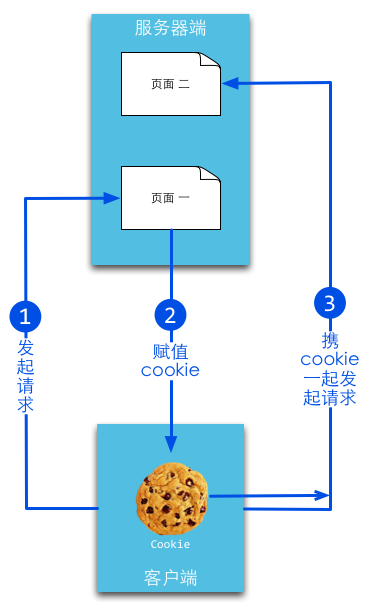
\includegraphics[width=7cm]{6.1.cookie2.png}
   \label{図6.1}
   \caption{cookieの原理図}
\end{figure}

sessionとは、簡単に言えばサーバ上に保存されたユーザの操作の履歴情報です。サーバはsession idを使用してsessionを識別します。session idはサーバが生成します。ランダム性とユニーク性を保証し、ランダムな秘密鍵に相当します。ハンドシェイクやデータ通信中にユーザの本当のパスワードが暴露されるのを防ぎます。しかしこの方法では、依然としてリクエストを送信したクライアントとsessionを対応させる必要があります。そのためcookieメカニズムによってクライアントのID(session id)を取得することで、GETメソッドでidをサーバに送信することができます。

\begin{figure}[H]
   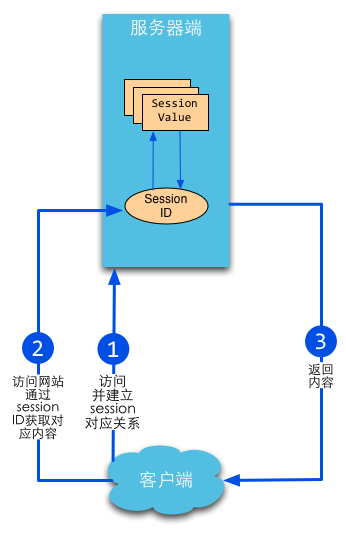
\includegraphics[width=7cm]{6.1.session.png}
   \label{図6.2}
   \caption{sessionの原理図}
\end{figure}



